%%%%%%%%%%%%%%%%%%%%%%% file template.tex %%%%%%%%%%%%%%%%%%%%%%%%%
%
% This is a general template file for the LaTeX package SVJour3
% for Springer journals.          Springer Heidelberg 2010/09/16
%
% Copy it to a new file with a new name and use it as the basis
% for your article. Delete % signs as needed.
%
% This template includes a few options for different layouts and
% content for various journals. Please consult a previous issue of
% your journal as needed.
%
%%%%%%%%%%%%%%%%%%%%%%%%%%%%%%%%%%%%%%%%%%%%%%%%%%%%%%%%%%%%%%%%%%%
%
%
\RequirePackage{fix-cm}
%
%\documentclass{svjour3}                     % onecolumn (standard format)
%\documentclass[smallcondensed]{svjour3}     % onecolumn (ditto)
\documentclass[smallextended]{svjour3}       % onecolumn (second format)
%\documentclass[twocolumn]{svjour3}          % twocolumn
%
\smartqed  % flush right qed marks, e.g. at end of proof
%
\usepackage{graphicx}
\usepackage{pbox}
\usepackage{hyperref}
\usepackage{booktabs} % For formal tables
\usepackage{xspace}
\usepackage{multirow}
\usepackage{hhline}
\usepackage{fancybox}
\usepackage{balance}
\usepackage{graphicx}
\usepackage{epstopdf}
\epstopdfsetup{outdir=./}



\newcommand{\hypobox}[1]{

        \begin{center}\noindent\thicklines\setlength{\fboxsep}{8pt}\cornersize{0.2}\ovalbox{

                \begin{minipage}{3.0in}

                        \textit{#1}

                \end{minipage}} 

        \end{center}} 

%
% \usepackage{mathptmx}      % use Times fonts if available on your TeX system
%
% insert here the call for the packages your document requires
%\usepackage{latexsym}
% etc.
%
% please place your own definitions here and don't use \def but
% \newcommand{}{}
%
% Insert the name of "your journal" with
\journalname{Empirical Software Engineering}
%
\begin{document}

\title{Deriving a Usage-Independent Software Quality Metric }
%\subtitle{Do you have a subtitle?\\ If so, write it here}

%\titlerunning{Short form of title}        % if too long for running head

\author{Tapajit Dey         \and
        Audris Mockus %etc.
}

%\authorrunning{Short form of author list} % if too long for running head

\institute{Tapajit Dey  \and Audris Mockus \at
            Department of Electrical Engineering and Computer Science \\  
            University of Tennessee, Knoxville \\
            Knoxville, Tennessee, USA \\
            tdey2@vols.utk.edu,  audris@utk.edu 
}

\date{Received: date / Accepted: date}
% The correct dates will be entered by the editor


\maketitle

\begin{abstract}
 Context: The way post-release usage of a software affects the number of
  faults experienced by users is scarcely explored due to the proprietary nature 
  of such data. The commonly used quality measure of post-release faults may, therefore, 
  reflect usage instead of the quality of the software development process.
 Objective: To determine  how software faults and software use are related in a 
  post-deployment scenario and, based on that, derive post-deployment quality 
  measure that reflects developers' performance more accurately.  
Method: We analyze
  Google Analytics data counting daily new users, visits,  time-on-site, 
  visits per user, and release start date and duration for two complex 
  proprietary mobile applications, one for iOS (General Availability 
  version) and one for Android (Development and General Availability versions).
  We utilize Linear Regression, Bayesian Network (a simulation exercise was performed
  for determining the best BN structure search method that was used during our analysis), and Random Forest 
  models to   explain the interrelationships and to derive release 
  quality measure that is relatively stable with respect to variations 
  in software usage.  We also present a timeline for observing when 
  the exceptions typically occur in the release duration. 
  We further extended our study and looked into 4430 NPM packages that had more than 10,000 
  monthly downloads (since January, 2018) and looked at the interaction between the number of 
  downloads and the number of issues reported against that package.
Results: We found the number of new users to be 
  the primary factor determining the number of exceptions, and found no
  direct link between the intensity and frequency of software usage and 
  software faults. Furthermore, the relative increase in the number of
  crashes was found to be associated with a power of around 1.02-1.04 relative increase
  in the number of new users for the android app, and around 1.6 for the iOS app. Based on the findings we
  propose a release quality measure: number of crashes per user for a 
  release of the software, which was seen to be independent of
  any other usage variables, providing us with a usage independent
  measure of software quality. From the study of the NPM packages we found that the
  number of downloads has a strong effect on the number of issues for almost all the packages.
  However, we found from the timeline analysis that for 45.8\% of the packages, the number of issues 
  per download increases with time, unlike for the releases of the mobile app where the exceptions per user 
  decrease with time for almost all releases.
Conclusions: We expect our result and our proposed quality measure will help
  gauge release quality of a software more accurately and inspire further 
  research in this area.

\keywords{Software Quality \and Software Usage \and Software Faults \and Bayesian Networks \and NPM packages}
% \PACS{PACS code1 \and PACS code2 \and more}
% \subclass{MSC code1 \and MSC code2 \and more}
\end{abstract}

\section{Introduction}\label{s:intro}

Improving quality of software is one of the objectives of software
engineering.  ``Software Quality'' has been defined in various ways,
but in this paper we take a narrow focus on the manifestation of software
defects as crashes observed from the perspective of the
users. Observing a software crash, generally speaking, a is
manifestation of low quality to a user of the software. 
Thus, it seems intuitive to measure the quality of software\footnote{in fact, we
  mean to measure one aspect of the quality of software}
by counting the number of crashes. More crashes would be associated
with lower quality. If, for example, we compare 
two different softwares or two different releases of a software,
we first calculate the number of crashes for each and then compare
these numbers. Software with more users, however, tends
to see more crashes~\cite{dey2018modeling,hmps15,IQ08} as each user
may exercise it differently. In
an extreme case, a software or a release with no users will have
no crashes, regardless of its quality. This interdependence of
software usage volume and crashes experienced is typically not
considered in quality measurement in industry or in empirical studies (although few studies
do note that~\cite{fenton2008using,fenton1999critique}).
Ignoring this relationship, however, would misguide quality
improvement efforts (avoid quality improvements for low usage
releases) and/or misguided developer
performance metrics (reward developers of low-usage products). This analogy can also be extended for software
defects (bugs) as well, and by extension for issues raised against a
software, since software crashes are manifestations of underlying
defects and~\cite{caper,hmps15} observed that the number of
discovered software defects increases with the number of users,
although the relationship between crashes and defects is not very
well understood~\cite{fenton1999critique}.  

One possible reason for this oversight is the scarcity of reliable usage data. While the number of defects and crashes reported by users are carefully tracked by most large scale projects (\textit{e.g.} Mozilla Firefox, Ubuntu etc.), tracking the variables related to usage, \textit{e.g.} the number of users, intensity of usage etc. is almost impossible to track without a reliable monitoring system. Such a system is rarely used by open-source softwares and even many traditional software-as-a-product systems do not or can not have such capability. Moreover, even when such a dataset is available, it is almost always proprietary, so obtaining and sharing it, even for the software development teams in these proprietary projects, is difficult since the deployment is typically managed by a different team within the organization. Without such data, however, it becomes exceedingly difficult to interpret the quality of a software from the customer reported crashes/defects alone due to the interdependence of usage and crashes/defects~\cite{dey2018modeling,hmps15,IQ08}.

We were able to obtain the usage data for several mobile applications developed by Avaya, \textit{viz.}  Avaya Communicator for Android (currently known as Avaya Equinox\textregistered) and Avaya one-X\textregistered  Mobile SIP iOS Client. The usage data was obtained from Google Analytics. By analyzing the usage data for these applications we establish the interdependence between the number of crashes and usage, and propose a quality metric that is independent of usage, which would enable us to compare the qualities of different softwares and/or different releases of a software more accurately. 

We used three usage related variables: number of users, 
usage intensity (average duration of software use per user), and usage frequency 
(average number of times the app was used by a user), along with two variables describing attributes 
of the particular release: release date and effective duration of the release, measured by how 
long the release continued to have new users, and looked at how these variables affect 
the number of exceptions \textit{i.e.} application crashes.  

After the usual data cleaning and variable construction stages, we first applied a linear regression (LR) model to identify the significant predictors for the number of exceptions. Then we used a Bayesian Network (BN) model to discover the interrelationship between the variables. The BN model was generated by using structure search algorithms, and the search method was chosen based on the result of a simulation study. We have presented the detailed result of the simulation study and hope that other practitioners willing to use BN structure search methods in their work might find it useful.  Finally, we ran a random forest (RF) model to identify the importance of the variables for predicting the number of exceptions. All analyses in this study was done in R~\cite{R}. We found that the frequency and intensity of usage have little impact on the number of exceptions, but the number of users does have a significant impact. 

In our previous work~\cite{dey2018modeling}, we only analyzed the General Availability releases for  Avaya Communicator for Android. Since the data was collected through similar means, we had the same set of variables for all the Avaya softwares. We found similar results from that study as well, with the number of new users being the most important factor affecting the number of exceptions.
Furthermore, we proposed a quality metric of average number of exceptions experienced by end users (so lower means better) and found it to be independent of other usage metrics. 

In this study, we have added the analysis of the development version of Avaya Communicator for Android and the
General Availability releases of Avaya one-X\textregistered  Mobile SIP iOS Client. Although we collected data for several other apps, those were dropped due to having too few releases/ exceptions/ users to give a reliable result. We employed the same set of analysis methods and found the result to be very similar for all cases considered and it matched our result of the previous analysis as well. We also added a timeline showing how the perceived quality of the releases vary with time for different releases.  

We have also applied our method of analysis to a very different scenario of NPM packages. Node Package Manager (NPM) is the package manager for node.js, an open-source, cross-platform JavaScript run-time environment. 
Since we do not have the number of crashes for these packages, we looked at the number of issues reported for these packages instead.
NPM tracks the number of downloads of the packages, and while the number of downloads counted by NPM is essentially a mix of downloads by users, bots, and mirror servers, as explained in~\cite{npmdl}, it is the closest measure of usage we could find for open-source projects. We only looked at the NPM packages that have more than 10,000 downloads a month. While according to ~\cite{npmdl}, automated downloads are expected to be around 50 per day, or 1500 per month, we wanted the usage to be high enough to have a noticeable impact on the number of issues reported, so we set the threshold to 10,000. We collected the issues associated to the projects from their individual GitHub repositories. We found 4430 projects which had more than 10,000 monthly downloads since January 2018 and also had public GitHub repositories with nonzero number of issues. 
We collected the number of downloads and the total number of issues for all these packages from 2015-03-01 to 2018-08-31. However, we did not conduct a release by release comparison for these packages, since the release durations vary by a lot for most packages. Since the recorded number of downloads is a mix of downloads by human and non-human users, a release by release comparison would not give a reliable picture of the effect of actual usage by human users on the number of issues. However, the number of downloads by bots are relatively stable and vary only with time, so controlling for the date would eliminate the spurious effects of downloads by bots. So, we decided to focus on the entire packages instead of releases of the packages, and measured the effect daily downloads have on number of issues of that package on that day after controlling for the calender date. 

From the analysis of NPM packages we found that for only 36 out of 4430 packages (0.8\%) the number of daily downloads is not a significant predictor (p-value $> 0.5$ ) of the number of issues on that day.

In summary, we have established the relationship between the number of exceptions (crashes) and usage by analyzing different softwares, and have proposed a Bayesian quality metric that gives a more complete and reliable measure of quality. We have also used our approach to study the relationship between the number of downloads and issues of 4430 NPM packages and found it to be a significant predictor for most (99.2\%) of them. We have also presented the detailed result of the simulation study we conducted to choose the best performing BN structure search algorithms, which we believe will of of use to practitioners willing to use BN structure search methods in their work.

The rest of the paper is organized as follows: In Section~\ref{s:relwork}, we discuss the related works and other studies that have found similar results. In Section~\ref{s:soft}, we give some details about both the commercial software and NPM packages we analyzed. Details of the data collected for the study is discussed in Section~\ref{s:data}. Section~\ref{s:datapre} lists the data preprocessing steps we followed. We discuss the simulation study we performed for choosing the best performing BN structure search method that was used in subsequent analysis in Section~\ref{s:sim}. In Section~\ref{s:explain}, we present the different modeling approaches used to explain the number of exceptions(crashes) for the commercial softwares we studied and the results of that study. A comparison of our result and already published results is presented in Section~\ref{sec:compare}. 
The quality metric we used is discussed in Section~\ref{s:qual}. The result of the analysis of the NPM packages is presented in Section~\ref{s:npm}. We discuss the implications of our result in Section~\ref{s:implication}. Finally, we discuss the limitations of our study in Section~\ref{s:limitation} and conclude the paper in Section~\ref{s:conclusion}.  

\section{Related Work}\label{s:relwork}

Although software quality has always been a common
topic in software engineering~\cite{boehm1976quantitative,kitchenham1996software}, most of
the studies have focused on pre-release data, primarily due to the
developers' concern about finding the appropriate balance between
the amount of testing required and the quality of software
(e.g.~\cite{rubin2016challenges,dalal1988should}). There have been a
number of works on predicting and improving the software quality as
well (e.g.~\cite{MHP13,zhang2015towards,KSAHMSU13,MW00}). Comparatively,
studies about post-deployment quality and dynamics have been less
frequent~\cite{li2011characterizing,kenny1993estimating}. However, a
number of studies have looked at the aspects of software quality
metrics, especially the quality perceived by the customers,
e.g.,~\cite{mockus2005predictors,IQ08,hmps15,rotella2011implementing,M14}. A notable
non-academic work involves a study of mobile app monitoring
company's (Crittercism) data~\cite{crittercism12}. The author of the
news article found it necessary to normalize crash data by the
number of launches. Finally, an empirical investigation between
release frequency and quality on Mozilla Firefox has been
investigated in~\cite{khomh2012faster}. 

While Bayesian Networks have been used for software defect prediction 
for decades, the use of BNs for explanatory modeling in
empirical software engineering is still not common despite the
promise. A case for use of BNs was made
by Fenton et.al.~\cite{fenton1999critique,fenton2002software}, while the earliest publications
utilizing BNs we could find~\cite{HM03a} constructed search of the
structure based on the statistical significance of partial
correlations in the context of modeling delays in globally
distributed development. \cite{stamelos2003use,pendharkar2005probabilistic} considered
the application of Bayesian networks to prediction of effort, 
\cite{fenton2007predicting,neil1996predicting,okutan2014software} 
used Bayesian networks to predict defects, and \cite{pai2007empirical} 
used BN approach for an empirical analysis of faultiness of a software. 
On the other hand, Bayesian structure learning is a big domain in itself 
with a wide range of algorithms, but its use in software engineering context 
is not very common.

Post-release defect density calculated as a proportion of users who experience an issue within a certain period after installing or upgrading to a new release has been proposed by~\cite{mockus2008interval,mockus2005predictors} as a measure of software quality.  Hackbarth et al.~\cite{hackbarth2016improving} also found the need to adjust defect counts in their proposed measure of software quality as perceived by customers. We propose a somewhat different measure of quality based on the number of exceptions per user. In general, software quality is a widely researched topic~\cite{kan2002metrics,kitchenham1996software,schulmeyer1992handbook} etc., but in our knowledge, this is the first model-based attempt to obtain a usage independent measure of software quality and the first attempt to model exceptions in mobile applications.

The NPM ecosystem is one of the most active and dynamic JavaScript ecosystems and~\cite{wittern2016look} presents its dependency structure and package popularity.~\cite{zerouali2018empirical} studies the dependency, specifically the lag in updating dependencies in various NPM packages while~\cite{abdalkareem2017developers} looked into the use of trivial packages as part of package dependencies for different NPM packages. 


The advancements proposed in this paper over the published work are focused 
on two primary areas: (1) study of the relationship between software faults and usage 
using \textbf{post-release} data in mobile application context, and (2) proposing a usage independent exception-based software quality metric based on our models.



\section{Software Studied}\label{s:soft}

For this study, we looked into two different types of software, which are vastly different in nature. The primary focus of the study is on the commercial software developed by Avaya for mobile applications, which are from the telecommunication domain. For external validation of the theory developed using this data, we looked into the NPM packages, which are mostly open-source JavaScript packages used in web-development. In this section, we provide some details about the two to help contextualize our study.

\subsection{The Mobile Applications developed by Avaya}
One of the software chosen for this study was Avaya Communicator for
Android and iOS (currently known as Avaya Equinox\textregistered ). It
integrates the mobile devices of the users with their office Avaya
Aura\textregistered communications environment and delivers mobile
voice and video VoIP calling, cellular call integration, rich
conferencing, instant messaging, presence, visual voicemail,
corporate directory access and enterprise call logs\footnote{\url{https://support.avaya.com/products/P1574/avaya-equinox-for-android}\\   \url{https://support.avaya.com/products/P1597/avaya-equinox-for-ios/All}}.

Another software we studies was the Avaya one-X\textregistered Mobile  SIP  for  iOS, which provides mobile communications for the iPhone, iPod touch, and iPad through a wireless-enabled SIP Avaya Aura\textregistered environment combining enterprise features with the convenience of a mobile endpoint for users on the go. The Avaya one-X Mobile\textregistered SIP for iOS appears as an end point in the Aura\textregistered environment\footnote{\url{https://support.avaya.com/products/P0949/avaya-onex-mobile-sip-for-ios}}.

Avaya is developing large, complex, real-time software systems that
are embedded and standalone products. Development and testing are
spread through 10 to 13 time zones in the North America, USA, Europe
and Asia. R\&D department employed many virtual collaboration tools
such as JIRA, Git, WIKIs and Crucible. Development teams use
Scrum-like development methodologies with a typical 4-week
sprint. We consider a 15+ year old software component, the so-called
Spark engine.  As a software platform, Spark provides a consistent
set of signaling platform functionalities to a variety of Avaya
telephone product applications, including those of third parties.
Spark is a client platform that provides signaling manager, session
manager, media manager, audio manager, and video manager. The
codebase involves more than 200K files and, over all forks, over 4M
commits.  The Android software chosen for this study is a fork of
the Spark codebase. A more in-depth description of the development
process is provided in~\cite{amhp14}.

\subsection{NPM Packages}
Node Package Manager or NPM is one of the most active and dynamic software ecosystems at present. It currently hosts more than 800,000 packages, and have more than doubled in size in past couple of years (in January 2017, NPM reportedly hosted around 350,000 packages~\cite{npmpkg}). The popularity of NPM packages have, accordingly, skyrocketed as well. According to~\cite{npmpop}, ``JavaScript is getting more popular all the time, and NPM is being adopted by an ever greater percentage of the JavaScript community." About 75\% of all JavaScript developers used NPM, with about 10 million users, in January 2018, according to~\cite{npmpop}. Therefore, NPM is an excellent candidate for this study. Moreover, since they track the number of downloads of all packages in the ecosystem, it can be used as a  measure of usage. Although the number of recorded downloads is a mix of downloads by actual users and bots, mirror servers etc.~\cite{npmdl} it is still a far better measure than, \emph{e.g.} number of stars of a GitHub repository which was used in studies like~\cite{borges2016understanding} as a measure of popularity, which is little different from usage as we measure it.



\section{Details of the Data}\label{s:data}

\subsection{Data on mobile applications collected from Google Analytics}
The post-deployment data for this application was obtained from the 
Google Analytics platform.
Google Analytics is a web analytics service offered by
Google that tracks and reports website traffic. It is now one of the most
widely used web analytics services on the internet. In addition to
traditional web applications it also allows tracking of mobile
applications. To do that, the producer of a mobile application needs
to set up an account and instrument their mobile application to send certain
events to Google Analytics. Notably, it works for the mobile
applications investigated in this study. 

We collected data for a number of mobile applications developed by Avaya from Google Analytics, but some of the datasets turned out to be unusable for this study, for reasons ranging from very low volume of collected data (\textit{e.g.} Avaya Communicator for Android - Experimental Releases) to zero recorded exceptions making an analysis impractical (\textit{e.g.} Avaya One-X\textregistered   ScsCommander ). The following datasets were found usable:
\begin{itemize}
    \item Avaya Communicator for Android - General Availability and Development versions.
    \item Avaya one-X\textregistered Mobile  SIP  for  iOS - General Availability versions.
\end{itemize}

The data was collected between December 2013 and May 2016, although the exact time varies across the applications. Although we are primarily focused on the General Availability (GA) versions, since only these versions are available for end-users, we also decided to look into the development version for Avaya Communicator for Android, since we have detailed data available for these versions and we wanted to see if it shows a different characteristics from the GA versions.  

The original data obtained from Google Analytics had measures for the variables 
listed in Table~\ref{t:measures}, aggregated at a per-day granularity, meaning 
that each entry in the original data table contained the measures for the numerical 
variables (marked with a $\dagger$ symbol in the table) for each unique combination
of date, application release version, operating system version, mobile device brand, 
category, and model. We had the same set of variable for all the applications listed above.

It is important to note that Google Analytics releases only
aggregate data even to developers of the application and limits the
number of REST API calls, so one can not, for example, retrieve
usage data for every calendar second or get exact time of the
events. The daily counts split by release version of
the application, OS version, and type of device, provided
sufficiently fine granularity for our analysis. 
\begin{table}
\caption{Measures available in the Original Data}\label{t:measures}
\begin{tabular}{|p{6.5cm}|p{4cm}|}\hline
Application Release Version & No. of exceptions$\dagger$\\\hline
Operating System version in the user's device &Date of record entry\\\hline
No. of fatal exceptions$\dagger$& No. of new visits$\dagger$\\\hline
No. of visits$\dagger$ & Time on site$\dagger$\\\hline
\pbox{6cm}{Details on user's mobile device:\\ brand, category(mobile or tablet) and model} & No. of new users$\dagger$\\\hline
No. of total users$\dagger$& Sessions per user$\dagger$\\ \hline
\end{tabular}
\vspace{-10pt}
\end{table}

\subsection{Data on NPM Packages}

We used the API provided by NPM for collecting daily downloads of the 4430 NPM packages we studied. (The API documentation is available in: \textit{https://github.com/npm/registry/blob/master/docs/download-counts.md}).

To obtain the metadata information for every package in NPM, we wrote a ``follower" script, as described in 
\\ \textit{https://github.com/npm/registry/blob/master/docs/follower.md}.
The output contained the metadata information for all releases of all packages in NPM. From this we extracted the URL of GitHub repositories of the packages. Some NPM packages do not have a valid GitHub URL, so those were dropped from subsequent analysis. Using the Rest API provided by GitHub we collected information on the issues for all these NPM packages. Finally, we used the issue creation dates to construct a dataset of the total number of issues per day. We used the total number of issues instead of the number of open issues because we are interested in the number of issues encountered by the users of the packages. Whether an issue is resolved or not depends on a number of factors, \emph{e.g.} the number of developers, the responsiveness of the developers, the number of packages managed by each developer, the complexity of the problem, most of which are unrelated to usage, so we decided using the total number of issues is a much more reasonable option.

Our final dataset for the NPM packages contained the number of recorded downloads per day and the total number of issues reported for that package until that day. The date range was from 2015-03-01 to 2018-08-31. 


\section{Data Preprocessing}\label{s:datapre}

This section contains the data cleaning, transformation, and variable 
construction steps undertaken prior to the application of the different modeling 
methods. The NPM data was relatively clean, so we did not employ any preprocessing 
techniques on the collected data for the NPM packages. 

\subsection{The Google Analytics data for the Mobile Applications}

\textbf{Removal of variables before aggregation: } Upon initial
investigation into the data, we found that no. of exceptions and
no. of fatal exceptions were exactly the same, as recorded by Google
Analytics, so we removed the no. of fatal exceptions from the
dataset. Only fatal exceptions were recorded for this application,
i.e., crashes that require a complete restart of the mobile
application and, potentially, may affect the operating system
itself.  This is not surprising since the bulk of the functionality
for the application was written in C$++$ and called from the mobile OS
via Native Interface.

We did not consider the variables related to mobile device
details and operating system versions because the
application, as noted above, was primarily written in C$++$ and the
user interface aspects that vary greatest among devices and versions
of OS were not likely to have influence. To validate that
assumption we investigated and found no
correlation of exceptions with either variable. 

\noindent
\textbf{Data correction:}
This additional prepossessing step was not a part of our previous study~\cite{dey2018modeling}.
We found during careful inspection of the data that some of the releases had non-zero number
of users but zero new users in the dataset. This obviously hints at some part of the data 
being missing. So, as a data correction step, we modified the number of new users so that 
in the chronological order of the data, the cumulative number of new users is never 
less than the number of users for a day.

\noindent
\textbf{Aggregating data to per-release granularity:}
We had some missing values in the data, however, most of the missing data was about the
mobile devices and since we didn't use them in our analysis, we got rid of that
problem by simply dropping the variables. Since our aim is to model the quality of the
different releases, we aggregated the data to a per-release 
granularity, from the the original data that was recorded in per-day granularity. 
The raw data contained 177 different GA releases. We dropped 4 of
them from further consideration because a significant
portion of observations were missing. The result of aggregation, however,
was two new variables: start date (first day for which we have a
record for that release) of a release, and end date (last date for
which we have a record for that release) of a release, which in turn
helped create another variable: duration of a release. We did
not to keep the end date in the final table, since duration and
start date can be used to compute the end date.

\noindent
\textbf{Verifying the correctness of Release date:}
The original data involves only the usage aspects and the version
information of the software. The project under consideration was
relatively new and it was one of the early attempts for the team to deploy
mobile software on Android and iOS. As such, not everything
was well documented and also was rapidly evolving over time  and no
record of the exact release dates for most of the releases was
available. We did manage to get release dates for some of releases
from Google Play Store/ Apple App Store, but not all the release dates  were
available.  For the releases with dates available on Google Play
Store/ Apple App Store, the official release dates from Avaya records, and the start
dates obtained from the data were either very close or exactly the
same, so we do not have a reason to doubt the dates obtained from the
data. 

\noindent
\textbf{Removal  of variables post aggregation:}
The numerical variables were aggregated to give a sum for each
variable. Upon further inspection, we found the number of users, new
users, visits, and new visits to be highly correlated. In the second
iteration, we removed the variable ``sessions per user'', because
aggregating it directly is meaningless, and we were not sure how it
was originally calculated by Google Analytics (was it a mean or
a median? were new users or total users counted?). We also removed
the ``total users'' and ``total visits'', because while summing up the
new users/visits for each day gives an accurate measurement of the total
number of new users/visits for a release, it is not guaranteed that
summing up total users/visits does the same due to possible double
counting the number of users/visits. 

\noindent
\textbf{Final list of variables:}
Keeping the goal of our study in mind, the variables we have after the initial cleaning 
steps give us necessary information for a model of post-release defects and software usage.
In our list of variables, we have the total number of exceptions \textit{i.e.} post-release defects. 
As for measures related to software usage, we have the total number of new users;
the ``Time.On.Site'' variable, normalized by the number of users of a release,
provides a measure for the temporal intensity of usage per user;
and the number of visits per user is a measure for the frequency of usage.
We also have two variables related to each individual release: the start date \textit{i.e.} the release
date gives a measure for the calender time of each release, and is useful in gaining insight
about if the number of post-release defects and software usage vary with time, and 
the duration of a release, which could have an effect on the number of exceptions
and the number of new users, since these variables were not normalized with duration.
Since we only have a limited amount of data, we restricted ourselves to use only 
these six variables.
Our final aggregated data table had the measures listed in Table~\ref{t:finalvarss}, 
with the corresponding variable names we used in the model enclosed in brackets. 

\begin{table}
\caption{Measures in the Aggregated Data Table}\label{t:finalvarss}
\begin{tabular}{|l|l|}\hline
\pbox{6cm}{\textit{Release variable} - Start Date \\for the release (Release.Date)} & \pbox{6cm}{\textit{Release variable} - Effective Duration \\of the release (Release.Duration)}\\\hline
\pbox{6cm}{\textit{Post-Release defects} - \\Total No. of exceptions (Exceptions)}  &  \pbox{6cm}{\textit{Usage variable} - Average\\ time on site per user (Usage.Intensity)}\\\hline
\pbox{6cm}{\textit{Usage variable} -Total\\ number of new users (New.Users)} & \pbox{6cm}{\textit{Usage variable} \\- No. of visits per user (Usage.Frequency)}\\\hline
\end{tabular}
\vspace{-15pt}
\end{table}

\noindent
\textbf{Log-transformation of variables:}
The release date was converted from the Date format to numeric format, which 
resulted in the values for the release date variable being represented by the 
difference in days from Unix time (counted from 1970-01-01).
We found that all of the variables under consideration
had a long-tailed distribution, so we took logarithm of them. Final distribution of the variables in available in our GitHub repository:\\ \url{https://github.com/tapjdey/release\_qual\_model}.


\section{Simulation Study for Selecting the Best BN Structure Search Method}\label{s:sim}

\subsection{Basics of Bayesian Network models}
Bayesian Network~\cite{koller2009probabilistic,scutari2010introduction} 
is a type of Probabilistic Graphical Model (PGM), which explicitly represents the
conditional dependency/independence as a directed acyclic graph where variables
represent nodes and dependencies represent links, and thus this
representation can be used as a generative model\footnote{A
  generative model specifies a joint probability distribution over
  all observed variables, whereas a discriminative model
  (like the ones obtained from regression or decision trees) provides a
  model only for the target variable(s) conditional on the predictor
  variables. Thus, while a discriminative model allows only sampling
  of the target variables conditional on the predictors, a
  generative model can be used, for example, to simulate
  (i.e. generate) values of any variable in the model, and
  consequently, to gain an understanding of the underlying mechanics
  of a system, generative models are essential.}.  
Bayesian Networks models can be useful in the context of Software Engineering research~\cite{fenton1999critique} due to having several advantages over
regression models. To be precise, regression analysis is a very
simple BN where there is one directed link from each independent variable
to dependent variable. BNs, therefore, can help with 
multicollinearity, a common problem with software engineering 
data~\cite{yu2002predicting,subramanyam2003empirical,briand2000exploring,Changes07}, 
that is present in our data as well, by linking independent variables. 

Another variety of PGM that we did not use in this paper 
(details in Section~\ref{s:limitation}) is the Markov random
fields that represent the interrelationships between variables 
as undirected graphs. They differ in the set of
independencies they can encode and the factorization of the
distribution that they induce~\cite{koller2009probabilistic}.

\noindent\\
\textbf{Bayesian Network Model construction:}
Despite the promises of BNs, they tend to be quite sensitive to data,
and operational data, is often problematic~\cite{M14,zmz15}. 
Careful preprocessing, therefore, is needed to ensure a 
reliable and reproducible result. Two primary ways to use BNs exist. With the first
approach the graph represents dependencies obtained from domain experts.
The graph may include prior distributions
about the parameters of the overall model. The data is then used to
calculate the posterior distribution and to make inference. The
second approach puts minimal a-priori assumptions about the model
and focuses on the search for the best graphical representation for a given dataset
(structure learning). This is an NP-hard problem~\cite{chickering1996learning},
but a number of different heuristic structure learning algorithms are
available. Due to the lack of any strong theory connecting the variables we are considering,
we decided to use the structure search method for BN model construction.
Since our goal is to find a Bayesian network model for the data, we didn't
examine the methods that do not result in a Directed Acyclic Graph
(DAG). We found that the \textit{bnlearn} package in R implements a wide range of BN searching
methods for continuous, discrete, or a mixed set of variables and
the corresponding families of scoring functions and also has a good number of examples.
These methods were also shown to be able to recover the underlying network for a 
protein-signaling-chain (in Biology) in~\cite{bnppt}. We, therefore,
use this package for our analysis. In addition to the methods
implemented in \textit{bnlearn} package, we investigated some 
methods from a few other packages which can be interfaced with
the \textit{bnlearn} package.

Due to the potential inconsistencies of the BN models, we performed our 
modeling in two stages. First, we considered all available BN structure 
methods in the \textit{bnlearn} package and ran a simulation based study to 
find the methods that are most accurate and then we used those methods on our 
data to create the final model.

\noindent\\
\textbf{Methods considered:}\\
The different BN structure search methods we considered are listed below:

\begin{itemize}
\item \textit{Greedy search algorithms}(HC)~\cite{nagarajan2013bayesian,bnppt}
\item \textit{Hybrid algorithms}(Hybrid)~\cite{nagarajan2013bayesian,bnppt}
\item \textit{Posterior maximization} using \textit{deal} package in R~\cite{bnppt,dealR} .
\item \textit{Simulated Annealing} using \textit{catnet} package in R~\cite{catnetR,bnppt}.
\item \textit{MAP (maximum a posteriori estimation) Bayesian Model Averaging} (MAP) ~\cite{nagarajan2013bayesian,bnppt}
\end{itemize}

All structure search algorithms try to maximize some form of a network score. 
Among the various scores available, BIC score is the suitable one when 
the goal is to create an explanatory model from non-informative prior models
~\cite{shmueli2010explain,sober2002instrumentalism}.
BIC score is used for discrete data while the Gaussian 
equivalent of BIC (bic-g) score is used for continuous data.

The results, structure and parameters resulting from a structure
search algorithm are often noisy, meaning that
different settings induce slightly different networks. To mitigate
this effect we use non-parametric bootstrap model averaging method
described in~\cite{friedman1999data}, which provides confidence
level for both the existence of edge and its direction. This enables
us to select a model based a confidence threshold. Authors
of~\cite{friedman1999data} argue that threshold is domain specific
and needs to be determined for each domain. For instance, a threshold of 
 0.95 indicates that  only the edges that appeared in more than
 95\% of the bootstrap optimized models were selected. 
 
Many applications of BNs discretize the data prior to applying
the structure learning methods, so we considered it as a possibility as well.
Using continuous data works best
when the random variables (possibly after a transformation) 
have Gaussian distribution. While using
discrete data does not require such assumptions, obtaining the optimal
discretization for a dataset is in itself an NP-hard
problem~\cite{chlebus1998finding}. Choosing a
sub-optimal discretization technique may result in spurious or
missed relationships, which can in turn result in incorrect
dependencies being reported in the resulting model. Given the pros
and cons of both types of methods, we use methods of both types for
our simulation study. As we are interested in creating a generative model, we had to
use a discretization method that is unsupervised. The basic problem
with commonly used supervised methods (\textit{e.g.} Chi-square, or
MDLP discretization algorithms) is that they optimize
discretization to improve explanatory power for 
a single response variable. This is not suitable for a 
PGM structure search, because we do
not know  which variables will be responses (have arrows
pointing to them) and which will be independent (have no incoming
arrows) {\em a-priori}. While some research on multidimensional
discretization methods exists~\cite{perez2006supervised},
we are not aware of any that have a robust implementation.

\noindent\\
\textbf{Simulation Study:}\\
\begin{figure}
\centering
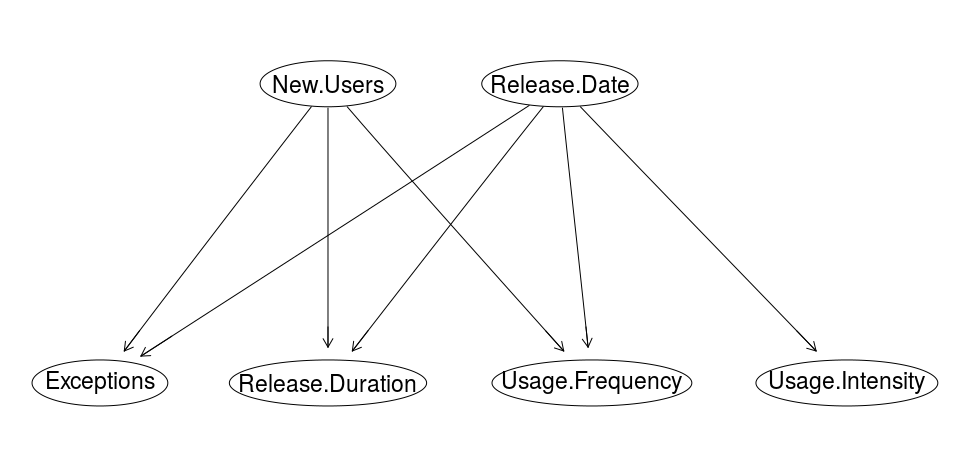
\includegraphics[width=\linewidth]{custom}
\caption{Custom model used for Simulation Study}
\label{fig:theory}
\end{figure}
We performed the simulation study by first creating 
a random BN (see Figure~\ref{fig:theory}) with 
six nodes, since we also have six variables in our final list (Table~\ref{t:finalvarss}).
For demonstration purposes we use the same variable names. 
We fitted this graph with our data (log-transformed and scaled) to generate values for the coefficients 
for each edge. This model was used in our simulation study going forward.
We created 1000 different datasets from the BN structure in Figure~\ref{fig:theory},
and applied the different structure search algorithms 
(both continuous and discrete versions, where available) listed above. Our performance metric
is finding how many times can the different algorithms recover the 
underlying structure from the simulated data. 

Other than testing the methods themselves, we also tested whether or not we should 
discretize the data. We tried different discretization methods, \textit{viz.} 
equal interval, equal frequency, and
k-means clustering based discretization methods from the
\textit{arules} package~\cite{arulesR}, and the 
Hartemink\footnote{Hartemink's pairwise mutual information 
method\cite{hartemink2001principled}.} discretization methods 
in the \textit{bnlearn} package.

Except for the \textit{Posterior maximization} using \textit{deal} package, 
all other results were bootstrapped, so we tested different thresholds in our 
simulation study as well. Finally, for the the Hybrid search algorithm, in which
conditional independence tests are performed to restrict
the search space for a subsequent greedy search, there are many restrict methods
available, \textit{viz.} gs" (Grow-Shrink), "iamb" (IAMB), "fast.iamb" (Fast-IAMB), "inter.iamb" (Inter-IAMB), "mmpc" (Max-Min Parent Children), "si.hiton.pc" (Semi- Interleaved HITON-PC), "chow.liu" (Chow-Liu), "aracne" (ARACNE)~\cite{bnlearnR}, and we tested all of these restrict options 
in our simulation study. 

\begin{table}
\caption{Result of Simulation Study}\label{t:sim_result}
\begin{tabular}{lll}
\hline
\textbf{Method} & \textbf{Exact} & \textbf{Off-by-one} \\ \hline
HC & 0.574 & 0.264 \\
MAP & 0.596 & 0.214 \\
Hybrid- si.hiton.pc & 0.000 & 0.019 \\
Hybrid- mmpc & 0.000 & 0.016 \\
Hybrid- gs & 0.000 & 0.011 \\
HC-D-F & 0.000 & 0.010 \\
Hybrid- iamb & 0.000 & 0.010 \\
Hybrid- mmpc -D-H & 0.000 & 0.008 \\
Hybrid- si.hiton.pc -D-H & 0.000 & 0.008 \\
HC-D-H & 0.000 & 0.007 \\
Hybrid- mmpc -D-F & 0.000 & 0.007 \\
Hybrid- si.hiton.pc -D-F & 0.000 & 0.006 \\
Hybrid- iamb -D-F & 0.000 & 0.005 \\
Hybrid- gs -D-F & 0.000 & 0.004 \\
Hybrid- gs -D-H & 0.000 & 0.004 \\
Hybrid- iamb -D-H & 0.000 & 0.002\\\hline
\end{tabular}
\end{table}

The result of the simulation study is shown in Table~\ref{t:sim_result}, which shows 
the fraction of times exact structures and off-by-one structures\footnote{one extra 
/ missing / reversed edge} were generated by each method in the simulation. The result varies 
with the chosen threshold, but in Table~\ref{t:sim_result}, we show the overall performance of
different methods and we only show 
the methods which generated an exact or off-by-one structure at least once in the simulation.
For the hybrid search methods, we list mention the restrict option that was used, and the 
`-D' suffix indicates a discretization method was used to discretize the data prior to applying 
a structure search method. `-D-H' indicates Hartemink discretization method and `-D-F' indicates 
Equal-Frequency discretization method. It is clear from the table that only HC and MAP methods
can effectively reproduce the correct underlying structure around half of the times and they create 
more off-by-one structures than others, indicating the error rate is the lowest for these methods.

\begin{table}
\caption{Result of Simulation Study: Different Thresholds}\label{t:sim_threshold}
\begin{tabular}{llll}
\hline
Method & Threshold & Exact & Off-by-one \\ \hline
MAP & 0.85 & 0.68 & 0.25 \\
MAP & 0.80 & 0.67 & 0.25 \\
MAP & 0.90 & 0.67 & 0.26 \\
MAP & 0.95 & 0.66 & 0.27 \\
MAP & 1.00 & 0.66 & 0.27 \\
MAP & 0.75 & 0.66 & 0.21 \\
HC & 0.65 & 0.63 & 0.23 \\
HC & 0.70 & 0.63 & 0.23 \\
HC & 0.75 & 0.63 & 0.23 \\
HC & 0.80 & 0.63 & 0.23 \\
HC & 0.85 & 0.62 & 0.24 \\
HC & 0.55 & 0.62 & 0.23 \\
HC & 0.60 & 0.62 & 0.23 \\
MAP & 0.70 & 0.62 & 0.21 \\
HC & 0.90 & 0.60 & 0.26 \\
MAP & 0.65 & 0.58 & 0.17 \\
HC & 0.95 & 0.57 & 0.29 \\
MAP & 0.60 & 0.43 & 0.14 \\
MAP & 0.55 & 0.33 & 0.11 \\
HC & 1.00 & 0.19 & 0.47\\ \hline
\end{tabular}
\end{table}

In Table~\ref{t:sim_threshold}, we show the fraction of times exact and 
off-by-one models were generated by HC and MAP methods for different thresholds. 
It can be seen that using a moderately high threshold between 0.75 and 0.9 gives
good results for both HC and MAP, while higher thresholds for HC and lower thresholds for MAP
give worse results. Using the optimal threshold creates models that have more than one wrong 
and/or missing edge only 7-14\% of the times. 

The result of the simulation study had the following findings:
\begin{itemize}
\item Using structure search algorithms on the continuous data resulted in much more frequent recovery of the original BN structure compared to discretized data.
\item Bootstrapping  improves the stability of the results considerably.
\item The bootstrapped Hill-Climbing search and MAP Bayesian Model Averaging algorithms outperformed all others both in terms of accuracy and runtime, being able to recover the underlying structure more than 63\% of the times and making no more than one error 86\% of times with optimal thresholds. 
\end{itemize}

We consider this study one of the contributions of the paper, and hope that it 
would be useful for researchers using BN structure learning techniques.

\section{Explaining Exceptions for the Commercial Software}\label{s:explain}
As mentioned earlier, we conducted our analysis in three stages: first, we used linear regression (LR) on the data with the number of exceptions as the response variable; then, we used Bayesian Network (BN) modeling approach to identify the interrelationship between the variables; and finally, we used a random forest (RF) model to verify the results. 

We chose LR for the simplicity, robustness and ease of interpretation. To better understand interrelationships among variable (since LR is not applicable for sets of highly correlated predictors) we used BN models. Finally, to establish the 
predictive capabilities of our models we used RF, which is known as one of the best Machine Learning classifiers. That way we could both obtain the most insight and also to validate our findings through the use of radically different approaches.

\subsection{Linear Regression Model}
We first used a linear regression model to discover the significant variables affecting the number of exceptions. The  output  of the fitted model is shown in Table~\ref{t:LR1}.The model resulted in a decent fit for the GA releases of Avaya Communicator for Android, given the sample size of 173, with adjusted $R^2$ of 0.481 (which is higher than  0.435, the adjusted $R^2$  reported with our previous approach~\cite{dey2018modeling}), and the variable ``New.Users'' was the most significant predictor while ``Release.Date'', ``Usage Intensity'', and ``Usage Frequency'' were also statistically significant. 

\begin{table}[ht]
\caption{Summary Result of LR model for ``Exceptions"}\label{t:LR1}
\centering
\resizebox{\columnwidth}{!}{%
\begin{tabular}{lrrr|rrr|rrr}
\hline
& \multicolumn{3}{c}{GA releases of Android} & \multicolumn{3}{c}{Dev releases of Android} & \multicolumn{3}{c}{Mobile SIP client for iOS}\\
  \hline
 & Estimate & Std. Error  & p-value  & Estimate & Std. Error  & p-value  & Estimate & Std. Error  & p-value \\ 
  \hline
(Intercept) & -145.7827 & 72.2447  & 0.0452 & -514.753 &  411.865 & 0.227 & 998.2528 & 284.0527 & 0.0170\\ 
  New.Users & 0.8172 & 0.1229 & 0.0000 & 1.08755  & 0.155 &  1.11e-06 & 1.2766 & 0.1969  & 0.0013\\ 
  Release.Date & 14.7756 & 7.4449 & 0.0488 & 52.884   &  42.383  & 0.227 & -103.8231 & 29.4034  & 0.0167 \\ 
  Release.Duration & 0.1361 & 0.1290 & 0.2930 & -0.031  &  0.297  & 0.917 & -2.0129 & 0.3381 & 0.0019\\ 
  Usage.Frequency & -0.5388 & 0.2179 & 0.0144 & -0.321  &  0.526  & 0.550 & 0.8246 & 0.9057  & 0.4043\\ 
  Usage.Intensity & 0.1261 & 0.0615  & 0.0419 & 0.025 &  0.183  & 0.892 & 1.0318 & 0.5286 & 0.1084\\ 
  \hline
\end{tabular}
}
\end{table}


\subsection{Bayesian Network Model}
One key assumption for applying the continuous BN structure search algorithms 
is that the variables have a distribution close to a Gaussian distribution.
To satisfy this modeling assumption, we scaled all the
variables to unit scale. The variable ``Exceptions" still had a long
tailed distribution, but the distributions of the other variables
were much closer to normal distribution.

According to the result of the simulation study, we decided to use bootstrapped hill-climbing search and MAP Bayesian model averaging methods for constructing the Final BN models for our datasets and considered the model that resulted from both the methods. 
The resultant BN model for the GA releases of Avaya Communicator for Android is shown in Figure~\ref{fig:finalAGA}.  Figure~\ref{fig:finalAD} shows the final BN Model for Development releases of Avaya Communicator for Android and Figure~\ref{fig:finalI} shows the final BN Model for GA releases of Avaya mobile SIP client for iOS.

Every bootstrap run was performed over 500 bootstrap samples, and a
hill-climbing search  with 100 random restarts was applied on each sample 
to find the best fitting network, so in essence, each resultant network was 
obtained by averaging 50,000 candidate networks. We used a Threshold of 0.85, as it seemed optimal from our simulation study.

\begin{figure}[!t]
\centering
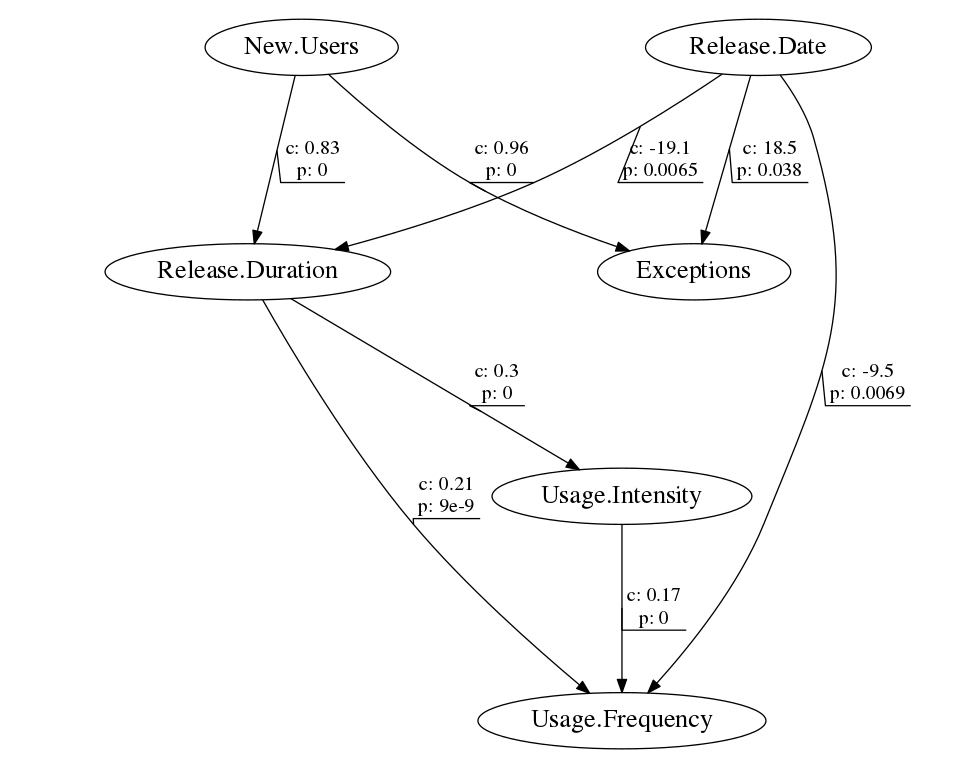
\includegraphics[width=0.7\linewidth]{AGA}%
\caption{Final BN Model for GA releases of Avaya Communicator for Android (with c: coefficients after fitting the transformed, but unscaled data, p: p-value  for the link) }
\label{fig:finalAGA}
\end{figure}

\begin{figure}[!t]
\centering
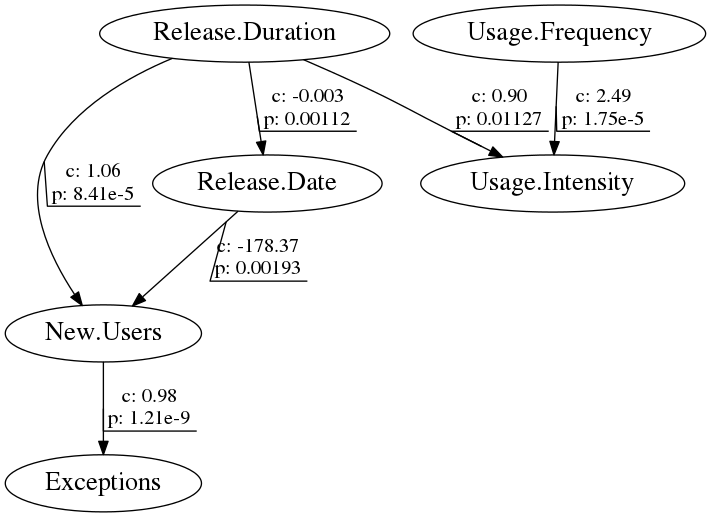
\includegraphics[width=0.7\linewidth]{AD}%
\caption{Final BN Model for Development releases of Avaya Communicator for Android (with c: coefficients after fitting the transformed, but unscaled data, p: p-value  for the link) }
\label{fig:finalAD}
\end{figure}

\begin{figure}[!t]
\centering
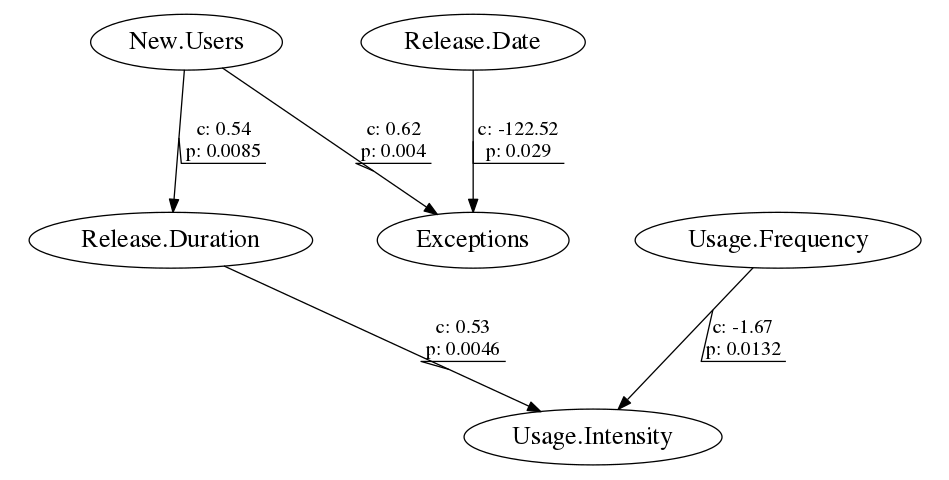
\includegraphics[width=0.7\linewidth]{i}%
\caption{Final BN Model for GA releases of Avaya mobile SIP client for iOS (with c: coefficients after fitting the transformed, but unscaled data, p: p-value  for the link) }
\label{fig:finalI}
\end{figure}

\begin{table}[ht]
\caption{Example bootstrap result - GA releases of Avaya Communicator for Android}\label{t:boot}
\centering
\begin{tabular}{llrr}
  \hline
 from & to & strength & direction \\ 
  \hline
Exceptions & New.Users & 1.00 & 0.34 \\ 
  Exceptions & Release.Date & 0.86 & 0.47 \\ 
  Exceptions & Release.Duration & 0.46 & 0.50 \\ 
  Exceptions & Usage.Frequency & 0.75 & 0.78 \\ 
  Exceptions & Usage.Intensity & 0.35 & 0.47 \\ 
  New.Users & Exceptions & 1.00 & 0.66 \\ 
  New.Users & Release.Date & 0.20 & 0.62 \\ 
  New.Users & Release.Duration & 1.00 & 0.71 \\ 
  New.Users & Usage.Frequency & 0.71 & 0.85 \\ 
  New.Users & Usage.Intensity & 0.34 & 0.64 \\ 
  Release.Date & Exceptions & 0.86 & 0.53 \\ 
  Release.Date & New.Users & 0.20 & 0.38 \\ 
  Release.Date & Release.Duration & 1.00 & 0.63 \\ 
  Release.Date & Usage.Frequency & 0.97 & 0.82 \\ 
  Release.Date & Usage.Intensity & 0.66 & 0.77 \\ 
  Release.Duration & Exceptions & 0.46 & 0.50 \\ 
  Release.Duration & New.Users & 1.00 & 0.29 \\ 
  Release.Duration & Release.Date & 1.00 & 0.37 \\ 
  Release.Duration & Usage.Frequency & 0.90 & 0.55 \\ 
  Release.Duration & Usage.Intensity & 1.00 & 0.53 \\ 
  Usage.Frequency & Exceptions & 0.75 & 0.22 \\ 
  Usage.Frequency & New.Users & 0.71 & 0.15 \\ 
  Usage.Frequency & Release.Date & 0.97 & 0.18 \\ 
  Usage.Frequency & Release.Duration & 0.90 & 0.45 \\ 
  Usage.Frequency & Usage.Intensity & 1.00 & 0.22 \\ 
  Usage.Intensity & Exceptions & 0.35 & 0.53 \\ 
  Usage.Intensity & New.Users & 0.34 & 0.36 \\ 
  Usage.Intensity & Release.Date & 0.66 & 0.23 \\ 
  Usage.Intensity & Release.Duration & 1.00 & 0.47 \\ 
  Usage.Intensity & Usage.Frequency & 1.00 & 0.78 \\ 
   \hline
\end{tabular}
\end{table}

The result form a bootstrap run shows the relative strength of the
link and the relative confidence for the direction of the link. 
In Table~\ref{t:boot} we have shown the result from one bootstrap run of the HC method for all possible edges for the GA release data of Avaya Communicator for Android. If an edge has $<50\%$ confidence in its direction, then the edge appears in the opposite direction in our model.
Although Bayesian Networks are sometimes interpreted as causal relationships~\cite{pearl2011bayesian}, there are disagreements on how that should be done.
We, therefore, are not interpreting these relationships as causal here. All observed links, therefore, indicate the presence of observed correlation (and are empirical in nature) and the direction is a property of the topological ordering of nodes in a DAG, and affects the total probability distribution of the variables.

The BN models were fitted to
the unscaled data, and the resulting coefficient of each link is also shown
in the figures. The p-value for each link was calculated from a
linear model with the source nodes as predictors and the destination
node as the response variable, e.g. the p-value for the link from
``New.Users" to ``Exceptions" was calculated by looking at the
result of:  \texttt{  lm(Exceptions $\sim$ New.Users $+$ Release.Date)}. \\
We fitted the model to the transformed, but unscaled data (for easier interpretation of results). 

By looking at the p-values for the links, we can say that all the links in the BN model
are statistically significant. 
Links having a negative coefficient indicate an inverse relationship between the parent 
and the child node.
The performance of explanatory models is evaluated by the fraction
of deviance explained by the model. Our model explains $45.5\%$ and $34.7\%$ of the
variation in ``Exceptions" (adjusted $R^2$ value of the model) for GA and development releases for Avaya Communicator for Android respectively and $20\%$ for GA releases of Avaya mobile SIP client for iOS. 


\subsection{Random Forest Model}
As a verification step to identify the important variables affecting the number of exceptions, we used a Random Forest model to fit the data, with ``Exceptions'' as the response variable. The variable importance plot for the GA release data of Avaya Communicator for Android, as shown in Figure~\ref{fig:rfAGA}, indicates that ``Release.Date" and ``New.Users'' are the two most important variables. We ran a 10-fold cross-validation exercise with ``Exceptions'' as the response variable, the resultant $R^2$ varied between 0.1176 and 0.6455 (mean: 0.4557, standard deviation: 0.1719). The high standard deviation is likely caused by our relatively small sample size of 173. This result reinforces the result we got from earlier analyses.

For the development releases of Avaya Communicator for Android, the variable importance plot is shown in Figure~\ref{fig:rfAD}. ``New.Users'' is again the most important variable, followed by ``Release.Duration''. 
For 3 out of the 10 folds, the $R^2$ value was negative, which basically means the fitted value had a different trend than the data~\cite{negRsq}. It varied between -3.15 and 0.89 (median: 0.06, mean: -0.22, standard deviation: 1.19)

For the GA releases of Avaya mobile SIP client for iOS, the random forest model resulted in very poor prediction performance, because the number of exceptions had little variation in the test set. However, the 
variable importance plot still shows the number of new users is the most important variable, as can be seen from Figure~\ref{fig:rfI}.

\begin{figure}[!t]
\centering
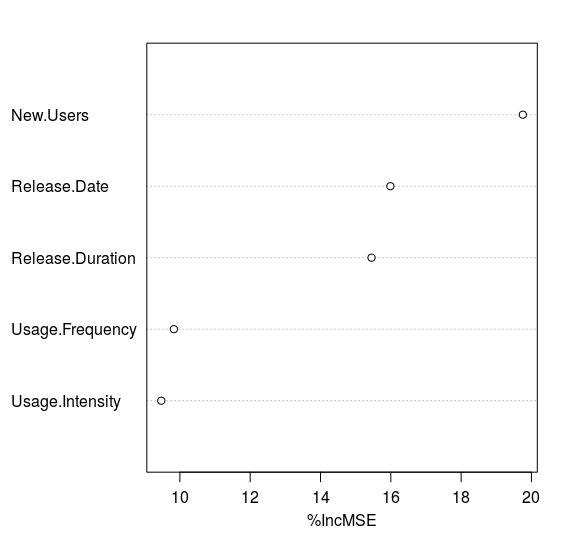
\includegraphics[width=0.4\linewidth]{rfAGA}%
\caption{Variable Importance Plot of RF model for ``Exceptions" for GA release data of Avaya Communicator for Android}
\label{fig:rfAGA}
\end{figure}

\begin{figure}[!t]
\centering
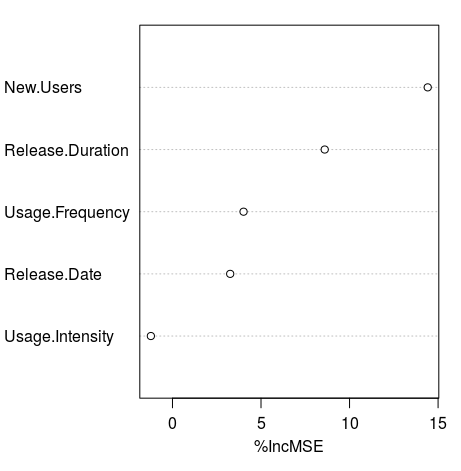
\includegraphics[width=0.4\linewidth]{rfAD}%
\caption{Variable Importance Plot of RF model for ``Exceptions" for development release data of Avaya Communicator for Android}
\label{fig:rfAD}
\end{figure}

\begin{figure}[!t]
\centering
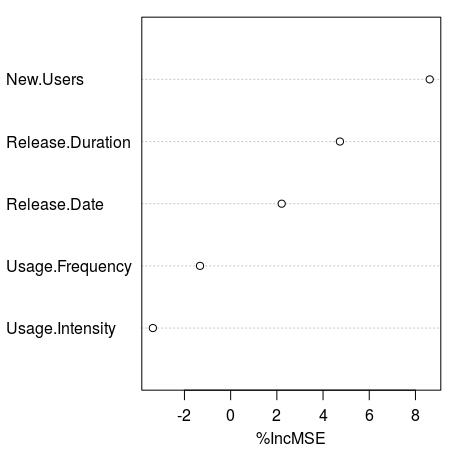
\includegraphics[width=0.4\linewidth]{rfI}%
\caption{Variable Importance Plot of RF model for ``Exceptions" for GA releases of Avaya mobile SIP client for iOS}
\label{fig:rfI}
\end{figure}

\section{Comparison with published results}\label{sec:compare}
In this section we compare our findings with already reported results that studied other commercial applications. 
The number of users for most of the releases we studied are very small, with a 
median of 7 users per release, although a few releases have more than 16,000 users.
On slide 22 of of his presentation~\cite{caper}, Caper Jones reported that the
number of defects increase 2 to 3 times for a 10 fold increase in the number of users
(from 1 to 10 and 10 to 100) for a software of similar complexity (between 10,000
and 100,000 function points). However, they were looking at the number of 
defects, and typically the number of 
exceptions is larger than the number of defects, because one defect could cause crashes for multiple users (or multiple crashes for a single user). The study published in~\cite{IQ08} was done for a system with many 
more users (around 4,000 to 16,000),however, they reported that for a two-fold increase in the 
number of users the number of Modification Requests (MR tickets) increase around $1.25$ times, 
which is less than what would have been predicted by our model ($1.78$). Although we
were unable to do a direct comparison to another mobile application, these findings add more context to our result, and indicates the necessity of further studies that publish their datasets to understand the usage-fault relationship in a wider range of applications.


\section{Application of our model: A derived measure of Quality}\label{s:qual}
In order to arrive at the usage independent quality measure, we follow the framework of establishing laws governing relationships among measures of software development proposed in~\cite{mockuskeynote}. Law is an equivalent of invariance, i.e. a function of measures that is constant under certain conditions. In this case we want it to be constant for releases that have the same quality. First, the law requires a plausible mechanism and second, an empirical validation. Each new user may have a different type of phone, operating system, service provider, geographic region, and usage pattern. It is reasonable to assume that some of these configurations lead to software malfunction manifested as an exception. This provides us with a plausible mechanism on how precisely more new users of one release might generate more exceptions even if we have two releases of identical quality. To obtain empirical validation of this postulated mechanistic relationship we rely on our models, all of which show the number of software 
exceptions to be dependent on the number of users and on software release date. Therefore,
we arrive at the following software law that is applicable for the investigated context: the average number of 
exceptions experienced by each user should, therefore, be independent of usage and depend only on the qualities of a software release.

In this section we test the above evidence-based hypothesis and provide the result of an analysis with the \textbf{number of exceptions per user} as a response variable (``Quality'') representing software quality. 
This is actually a measure for faultiness, so a lower value of ``Quality" indicates the actual quality of the software perceived by end users is better.

The value of the ``Quality'' variable (not log transformed) was seen to be varying between 0 and 10.85 (mean: 0.45, median: 0, standard deviation: 1.48) for the GA release data of Avaya Communicator for Android, between 0 and 22.83 (mean: 1.12, median: 0, standard deviation: 4.55) for development versions of the same, and for the GA releases of Avaya mobile SIP client for iOS it varied between 0 and 0.5 (mean: 0.0488, standard deviation: 0.15) . %%%%%

Similar to the previous analysis, we applied Linear Regression, Bayesian Network search, and 
Random Forest modeling approaches on the dataset containing this quality measure and the remaining variables, all of which were log-transformed. 

The result, as expected, shows that the quality of a software, measured by average number of faults experienced by each user, has no dependence on other usage variables. 
The LR model of GA releases of Avaya Communicator for Android (Table~\ref{t:lr2}) suggest that other variables have some effect on the quality variable.
The BN model(Figure~\ref{fig:bn2AGA}), obtained with a threshold of 0.85 from a bootstrapped Hill-Climbing structure search model, indicates the ``Quality'' variable depends only on  the ``Release.Date'' variable.
Finally, the result of 10-fold cross-validation with the RF model (Variable Importance plot in Figure~\ref{fig:rf2AGA}) indicates that the ``Release.Date'' variable is much more important compared to others, and the two usage related variables are of much lower importance. The $R^2$ value for the LR model was 0.1455 in this case, and for the 10-fold cross-validation (RF model) it varies between -3.368 and 0.643 (mean: -0.292, standard deviation: 1.371). The implication of negative $R^2$, as mentioned before is that the fitted model shows a very different trend~\cite{negRsq}.

For the development versions of Avaya Communicator for Android, the ``Quality'' variable turns out be insignificant in both the LR (Table~\ref{t:lr2}) and the BN (Figure~\ref{fig:bn2AD}) models. The RF model gives a really bad fit in the 10-fold cross-validation as well, with $R^2$ values ranging from negative infinity to 0.64 (median: -5.74), indicating the predictors are very poor. Still, the two usage related variables have the lowest importance in the variable importance plot as seen in Figure~\ref{fig:rf2AD}.

Finally, for the GA releases of Avaya mobile SIP client for iOS, the LR model shows that release date and release duration have effect on the ``Quality'' variable (although ), but the two other usage variables have no effect (Table~\ref{t:lr2}) and the BN (Figure~\ref{fig:bn2I}) models. The RF model again gives a really bad fit in the 10-fold cross-validation, with $R^2$ values ranging from negative infinity to -36.43, indicating the predictors are very poor. Still, the two usage related variables have the lowest importance in the variable importance plot as seen in Figure~\ref{fig:rf2I}.

\begin{table}[ht]
\vspace{-10pt}
\caption{Summary Result of LR Model for ``Quality"}
\label{t:lr2}
\resizebox{\columnwidth}{!}{%
\begin{tabular}{lrrr|rrr|rrr}
\hline
& \multicolumn{3}{c}{GA releases of Android} & \multicolumn{3}{c}{Dev releases of Android} & \multicolumn{3}{c}{Mobile SIP client for iOS}\\
  \hline
 & Estimate & Std. Error  & p-value  & Estimate & Std. Error  & p-value  & Estimate & Std. Error  & p-value \\ 
  \hline
(Intercept) & -59.6470 & 19.9155  & 0.0032 & --285.0676 & 180.0109 & 0.1290 & 28.5606 & 1.1271 &  0.0000\\ 
  Release.Date & 6.1428 & 2.0503  & 0.0031 & 29.3616 & 18.5247 & 0.1287 & -2.8833 & 0.1167 & 0.0000\\ 
  Release.Duration & 0.0514 & 0.0271  & 0.0600 &  0.0854 & 0.1152 & 0.4671 & -0.0923 & 0.0012 &  0.0000\\ 
  Usage.Frequency & -0.1593 & 0.0618  & 0.0108 & -0.3136 & 0.2372 & 0.2011 & 0.0006 & 0.0037 &  0.8831\\ 
  Usage.Intensity & 0.0395 & 0.0175  & 0.0253 & 0.0595 & 0.0820 & 0.4764 & 0.0001 & 0.0022 &  0.9614\\ 
  \hline
\end{tabular}
}
\end{table}


\begin{figure}[!t]
\centering
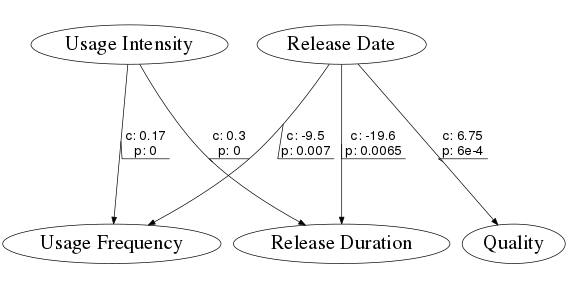
\includegraphics[width=0.6\linewidth]{qAGA}%
\caption{Bayesian Network  Model for ``Quality" - GA releases of Avaya Communicator for Android (with c: coefficients after fitting the transformed, but unscaled data, p: p-value  for the link)}
\label{fig:bn2AGA}
\end{figure}

\begin{figure}[!t]
\centering
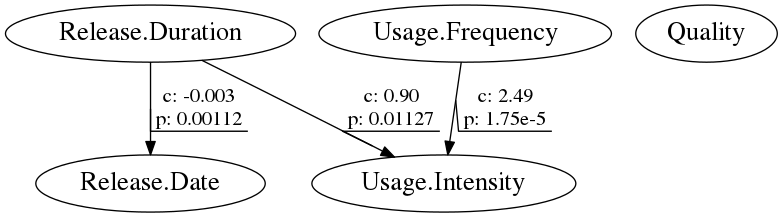
\includegraphics[width=0.6\linewidth]{qAD}%
\caption{Bayesian Network  Model for ``Quality" - Development releases of Avaya Communicator for Android (with c: coefficients after fitting the transformed, but unscaled data, p: p-value  for the link)}
\label{fig:bn2AD}
\end{figure}

\begin{figure}[!t]
\centering
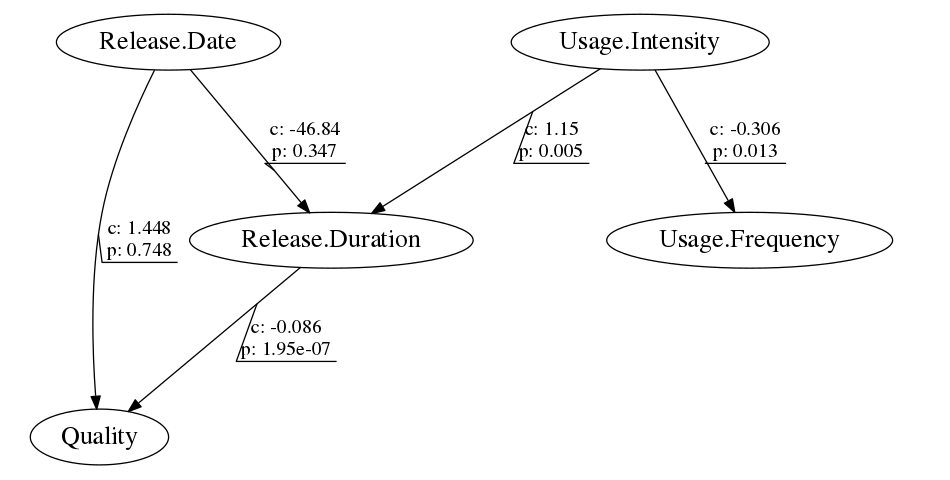
\includegraphics[width=0.6\linewidth]{qI}%
\caption{Bayesian Network  Model for ``Quality" - GA releases of Avaya mobile SIP client for iOS (with c: coefficients after fitting the transformed, but unscaled data, p: p-value  for the link)}
\label{fig:bn2I}
\end{figure}


\begin{figure}[!t]
\centering
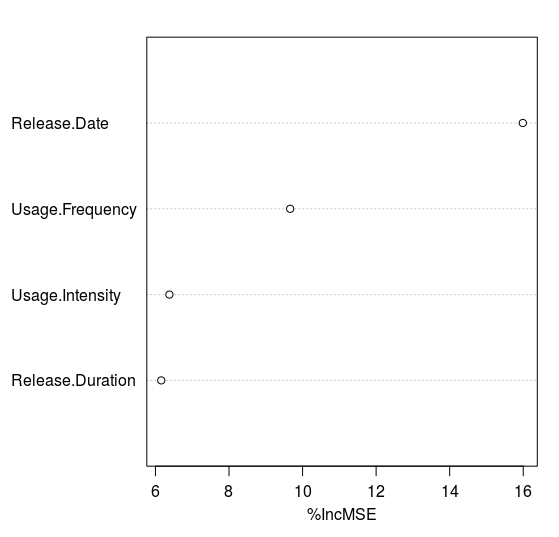
\includegraphics[width=0.4\linewidth]{rfqAGA}
\caption{Variable Importance plot from the Random Forest  Model for Quality Variable - GA releases of Avaya Communicator for Android}
\label{fig:rf2AGA}
\end{figure}

\begin{figure}[!t]
\centering
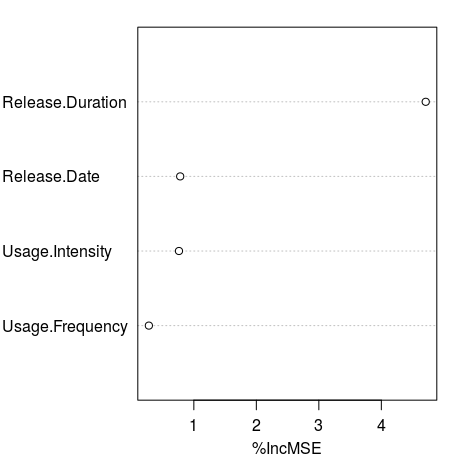
\includegraphics[width=0.4\linewidth]{rfqAD}
\caption{Variable Importance plot from the Random Forest  Model for Quality Variable - Development releases of Avaya Communicator for Android}
\label{fig:rf2AD}
\end{figure}

\begin{figure}[!t]
\centering
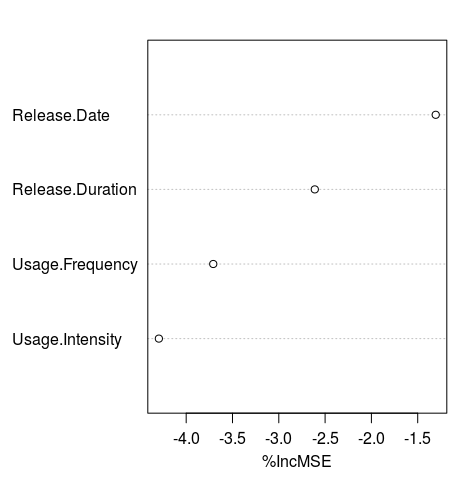
\includegraphics[width=0.4\linewidth]{rfqI}
\caption{Variable Importance plot from the Random Forest  Model for Quality Variable - GA releases of Avaya mobile SIP client for iOS}
\label{fig:rf2I}
\end{figure}

The results from these analyses clearly indicate that the quality measure defined by the number of exceptions per user is independent of software usage, and, therefore, suitable for comparing the quality of software development process among different releases of a software.

\subsection{Timeline of Quality}
We wanted to see how the perceived quality of the releases of the different mobile applications described above change with time. As a general trend, we observe that most of the exceptions occur right after the release date. then, as the number of users keep increasing with time, the value of the quality variable drop and come to a stable value.  In this paper we show only the timeline for GA releases of Avaya Communicator for Android (Figure~\ref{fig:tI}), since the other two softwares had a lot of releases, making them difficult to identify from the plot. The other two are added as supplemental material. %%%%%

\begin{figure}[!t]
\centering
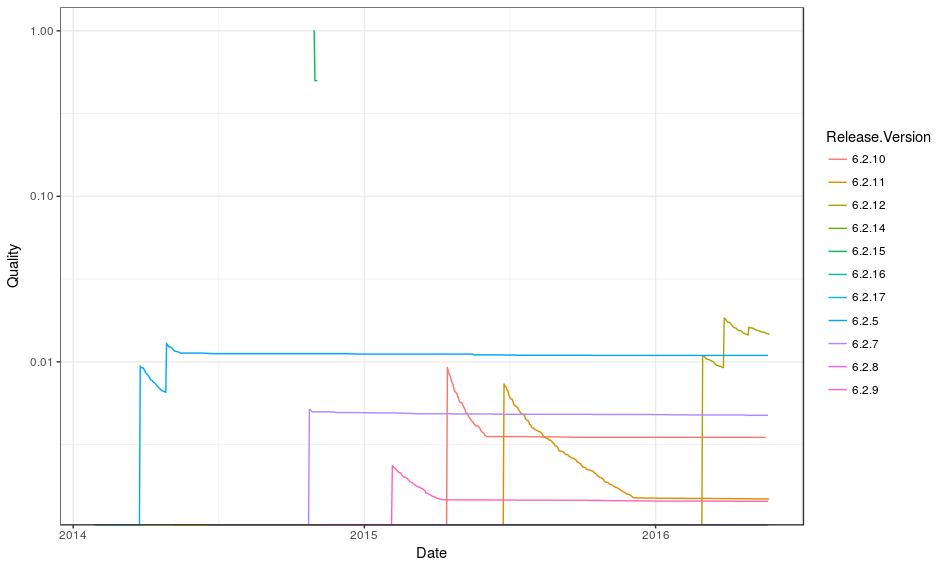
\includegraphics[width=\linewidth]{timeline_I}
\caption{Timeline for Quality Variable - GA releases of Avaya Communicator for Android}
\label{fig:tI}
\end{figure}



\section{Analysis of the NPM Data: Results}\label{s:npm}

As mentioned before, for the analysis of the NPM data we focused on the timeline of the entire packages, instead of the individual releases of a package to reduce the effect of the downloads by bots and other automated sources. Since we had only three variables in our dataset, we decided to go for the simpler liner model. We had the total number of reported issues for the package as the response variable and observed how much the number of daily downloads, before and after controlling for the calender date, explained it. 

We found that out of the 4430 packages, only for 36 packages the p-value of the predictor variable was more than 0.05 before adjusting for the calender date, and after adjusting for the calender date, p-value was less than 0.5 (\emph{i.e.} the predictor was deemed significant) for all 4430 packages. 

The $R^2$ values of the fitted models varied between 0 and 0.8637 (median: 0.4982, standard deviation: 0.0618) before adjusting for the calender date , and between 0.019 and 0.999 (median: 0.9195, standard deviation: 0.0618) after  adjusting for the calender date. So, we can say that the number of daily downloads is a significant and important predictor for the number of issues encountered by the users for most of the packages. 

Since we just established that the number of issues of an NPM package depends on the number of daily downloads, a similar quality metric of number of issues per download should be applicable in this situation as well. 

By calculating the quality metric in this way, we found that for different packages, it varied between 1.789 and 3531 (median: 12.755, standard deviation: 344.54). Further inspection showed that the value of the quality variable increases with time for almost half of the packages (2030 out of 4430 packages, 45.8\%), unlike what we observed for the mobile applications, where for almost all of the releases of the three softwares, the value of the quality variable decreased with time. 

Here we show the timelines of the quality variable we defined (\emph{i.e.} in this case, number of issues per download) for a few selected well-known NPM packages for illustration. We see that ``angular''(Fighure~\ref{fig:tNa}) and ``eslint''(Fighure~\ref{fig:tNe}) have a trend similar to what we saw for the mobile apps, with the value of the quality variable decreasing with time, but ``babel''(Fighure~\ref{fig:tNb}) is showing an increase in the value, while for ``ember-cli'', the trend is overall constant over time.

\begin{figure}[!t]
\centering
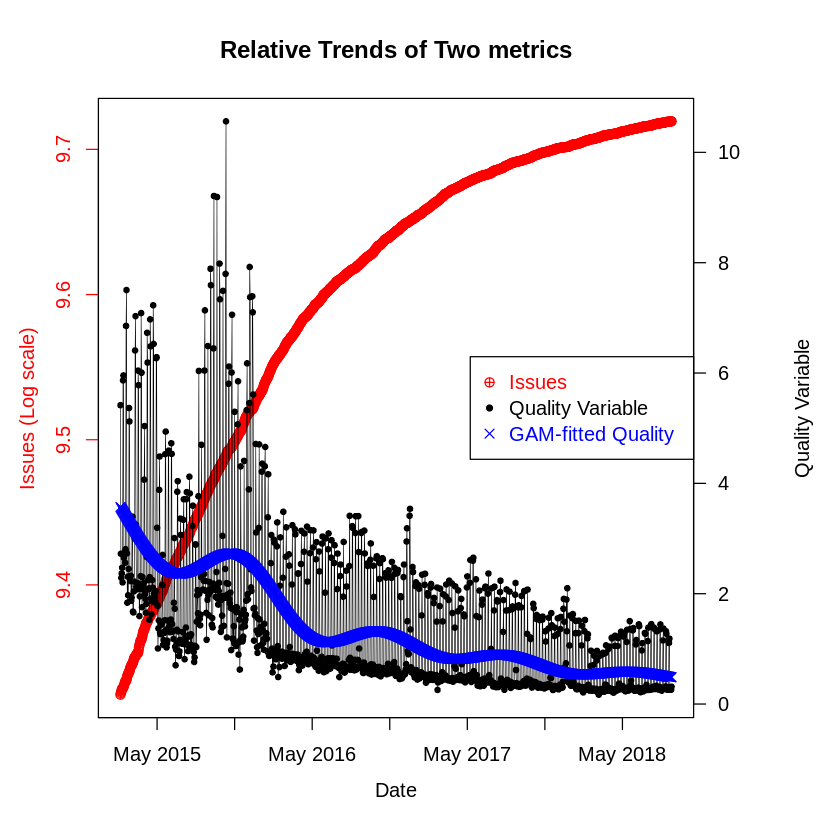
\includegraphics[width=0.5\linewidth]{angular}
\caption{Timeline for Quality Variable for NPM package: angular}
\label{fig:tNa}
\end{figure}

\begin{figure}[!t]
\centering
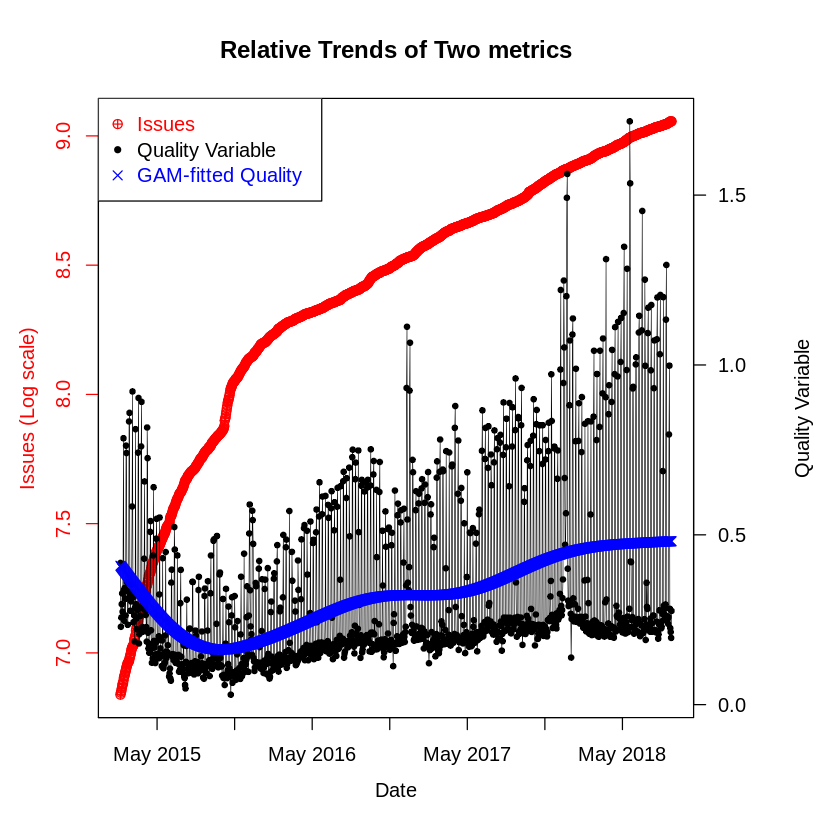
\includegraphics[width=0.5\linewidth]{babel}
\caption{Timeline for Quality Variable for NPM package: babel}
\label{fig:tNb}
\end{figure}

\begin{figure}[!t]
\centering
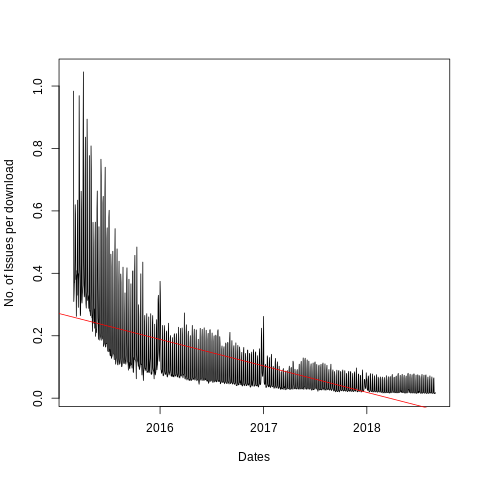
\includegraphics[width=0.5\linewidth]{eslint}
\caption{Timeline for Quality Variable for NPM package: eslint}
\label{fig:tNe}
\end{figure}

\begin{figure}[!t]
\centering
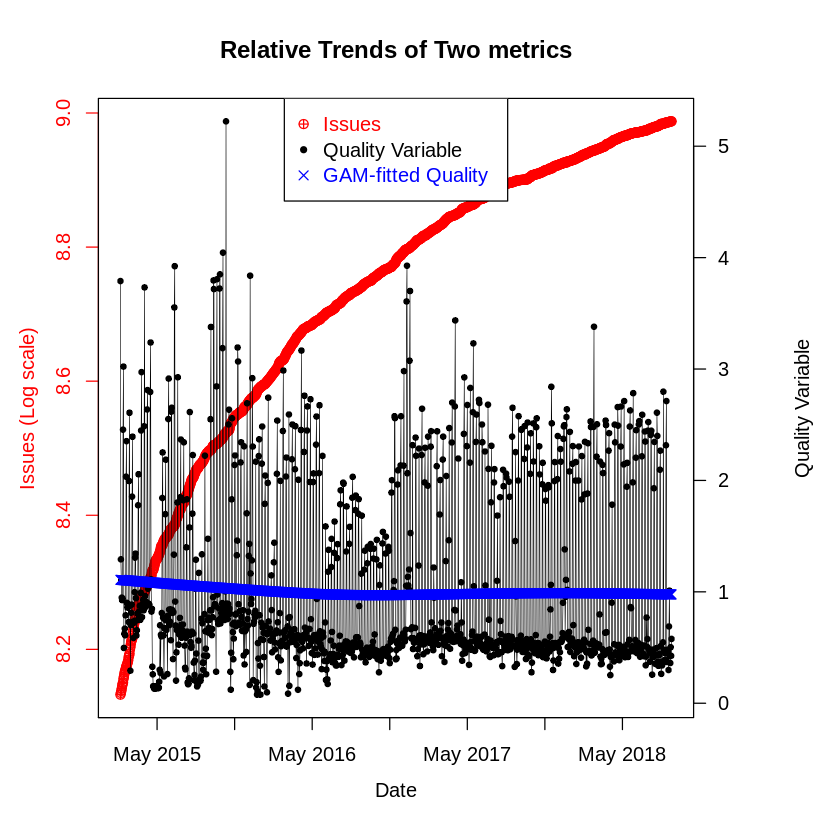
\includegraphics[width=0.5\linewidth]{ember-cli}
\caption{Timeline for Quality Variable for NPM package: ember-cli}
\label{fig:tNe}
\end{figure}


\section{Implication of our Findings}\label{s:implication}

Our analysis makes it evident that the number of new
users  is the most important variable in explaining various post-release variables, as seen in all three of the mobile applications as well as for the NPM packages. 
The analysis also indicates that more new users for a release indicate 
more exceptions being found for the software
and, for the GA releases of both the apps analyzed, longer activity for the release (the duration
of a release measures how long a release is actively used by users,
not the time between two releases, since the releases overlap).  This
suggests that users  may 
 be reluctant to upgrade (or are encouraged to stay) on better-quality releases.
 Our findings are in agreement with findings
of~\cite{IQ08,hmps15,mockus2005predictors} that consider 
post-release defects for a completely different server software system.

The release date also affects no. of exceptions, as can be observed by looking 
at the coefficients. It provides some insight on
how this software has evolved.  
Even after compensating for the effect the number of
users have on the number of exceptions, the number of exceptions are
increasing with time for the Android app, whereas is decreases for the iOS app. 
This may indicate that as the software, the OS, as well as the hardware are becoming 
more complex with time, which is consistent with a rapid growth of
functionality and the size of associated code base, the Android app is seeing more crashes due to the variations in the devices and the OS, whereas for iOS, since the devices as well as the OS versions are tightly controlled, the users are seeing less issues,   although we have no explicit evidence to support our speculation. 

We found from the timeline that, as a general trend, most of exceptions occur very early after the release, then as the number of users increase, the perceived quality of the release improves as well.


An interesting observation from the model is the lack of any direct relationship 
between exceptions and the intensity or frequency of usage.
One possibility is that exceptions happen for specific Android/
iOS version/ Phone combination and the way each user is exercising application's
functionality. Users for whom the application crashes must wait for
the next release. This would lead to the observed phenomena where
only the new users increase the number of crashes, which was observed more 
clearly from the timeline of crashes as well. The duration 
an application is used by individual users was found to have a much
smaller effect on reported defects than the number of
new users in prior work~\cite{hmps15,IQ08,MZL05} as well. In particular, it was observed
that most of the issues happen soon after deploying the release 
and the chances of reporting a defect for a new release drops 
very rapidly with time after installation.

We observed that for the NPM packages we analyzed, the number of downloads is a significant predictor for the number of issues for  most of the NPM packages, so a similar quality measure was used for this case as well. 
However, unlike the three mobile apps, where the value of our quality metric decreases with time for all releases, for the NPM packages the quality metric sometimes increases or remain relatively constant over time (around 45.8\% of the time). 

Our data, scripts, and more detailed results are available in our GitHub repository: \url{https://github.com/tapjdey/release\_qual\_model}.

\hypobox{%Aim 1 - key revelations:\\
We found that the exceptions are a result of more new users and the extent
of usage does not appear to have a direct effect on the number of new users.
}
 
Overall, none of the three models indicate that ``Usage.Frequency'' or ``Usage.Intensity'' have any effect on the ``Quality'' variable. We, therefore, suggest that the exceptions per new user can be used as a software development quality metric to compare quality of different releases and to quantifying the impact of variables representing the development process of a release.


\section{Limitations}\label{s:limitation}

In terms of modeling aspects, there are some limitations related to the different approaches.
 The RF model was used for 10 fold cross-validation, and exhibited a rather high value of standard deviation in the $R^2$ value, and it even went negative a few times indicating a very bad fit~\cite{negRsq},  likely due to the small sample size and not having good predictors in some models.

While creating the BN model we did not cover all possible ways BNs can be applied to gain insight into the system. For example, we did not investigate the possible existence of any hidden node, or make an effort to formally establish the causal relationship between the nodes. We also did not investigate how the properties of one release affect the subsequent releases, nor did we investigate the presence of any feedback loops.

In the simulation study, although we covered an extensive set of options, we did not try every possible combination of options for the BN structure search exercise.

We also did not use Markov Random Field analysis, which is another probabilistic graphical modeling approach. The primary reason behind choosing the BN approach was that we found an example where this method was used to successfully recover the underlying network~\cite{bnppt}. 
Moreover, it is possible to interpret a BN model as a causal model, and although we did not use that interpretation in this study, our goal is to eventually establish a causal mechanism of how usage affects the number of exceptions/defects experienced by users, so we wanted to used BN from the start.


The accuracy of our result is very much dependent on the Google
Analytics data. While we do not have reasons to doubt the accuracy of
the counts in Google
Analytics data, we would have liked to have better definitions of
how it determines ``New User'', ``Visit'', and, especially,
nontrivial to aggregate quantities such as ``Visits per User.'' Also,
it is not clear if Google
Analytics distorts data in any way (e.g., by applying differential 
privacy transformations) for low counts in order to protect
the privacy of the users. We do not believe it does, but we have not
conducted an experiment to validate that. 

Furthermore, the projects under consideration were relatively new and
it was the first attempt for the team to deploy mobile software. As
such, much was not well documented and was rapidly
evolving over time. As mentioned earlier, we did not have the official release
dates for all releases, so we put the start date of the release as
the date on which the first usage was reported. However, we did
verify the official dates with this reported date for the releases
for which we found the release date, and they were very close, but
not always exactly the same. This should not affect
the overall result, given the total time scale of more than two
years. The release end dates, by their nature, have to be estimated 
based on user activity, since there is no way to force end user
to upgrade Android app. For recent releases, therefore, the end date 
may be censored by our data
collection date, hence the duration for these releases might be
underestimated. 

It may be possible to collect numerous additional variables that may
have an impact on exceptions, for example, the number of changes to
the source code made for a release as was done
in~\cite{IQ08}. Unfortunately, due to the nature of parallel
development for multiple releases and products noted in
subsection~\ref{sub:soft}, it was virtually impossible to separate
the changes that would only affect the specific release on the Android
platform. There might be other unobserved variables driving some
relationships, but not explored in this study. 

Our model is obtained on a single set of mobile applications 
from a specific domain, implemented via
a rather complex codebase and is certainly not representative of
most mobile applications that tend to be much simpler. Furthermore,
mobile applications  
may not represent other types of software further limiting external
validity of the results. However, some aspects that we see in the
specific application, such as increasing number of faults with the
number of users, has been observed in rather different contexts of
large-scale server software. This suggests that the model derived in
the study may generalize to other domains as well. 

The study of the NPM packages was rather limited in scope, since we
only looked at the popular (having more than 10,000 monthly downloads 
since January 2018) packages to reduce the effect of downloads by 
automated sources. We didn't look at the effects of other factors 
that affect the number of downloads, \emph{e.g.} the number of 
dependents a package has. Although some of the issues could come 
from users of a dependent package, we didn't actively check the
origins of the issues to verify that. We also didn't look at the
releases of the packages, because of reasons mentioned before.
We didn't differentiate between the types of the issues, because we 
just wanted to see how many times a user decided to file an issue.
Overall, this study was not a direct extension of the previous work,
rather, it was an extension of the concept and its application in a different domain.



\section{Conclusion}\label{s:conclusion}

From the practical perspective we have established
that the extent of use has very strong relationship with the number
of exceptions for three large mobile applications from 
the telecommunication domain. Counting exceptions,
therefore, will not accurately measure the quality of software
development process but, instead, it would strongly depend on the
extent of use. In order to produce a measure that the development
team can use to understand and improve quality of their software
development process, we proposed to normalize exceptions by usage
based on the Bayesian Network models. Notably, a similar
normalization was previously proposed in the context of post-release
defects that also exhibited strong positive correlation with the
number of users.  As a larger proportion of applications are mobile
and/or delivered as a service, the amount of usage can be relatively
easily be collected.  Consequently, not adjusting software
development measures for usage should not be considered as an
excusable practice.

From the theoretical perspective we provided the explanation of the
relationships among post-deployment quantities using Linear
Regression and Bayesian Networks. Linear Regression can be thought
as a special Bayesian Network with the response node being
potentially connected to each predictor node. Bayesian Networks
allow for exploration of relationships among all variables and
empirical determination of the relationships exhibited in a
particular dataset.  Both models indicate that there are only two
variables that are related to exceptions in this data: number of
users and release date which we used as a proxy for the release
quality. It would be preferable to have each release as a separate
categorical predictor, but because for simplicity we chose to use
only one observation per release, it could not be done. If, instead,
we considered exceptions during different periods of a release, that
would have allowed us to introduce such categorical variable and
interpret the estimated coefficient for each release as release
quality (higher number meaning lower quality).

We also established
that it is possible to predict exceptions using Random Forest
modeling techniques and that usage plays a key role for the accuracy
of these predictions. As noted above, prediction is a different task
than explanation and, even though it often yields more accurate
results, the prediction results may be harder to explain to
developers or managers and, therefore, harder to act upon. We
believe the findings do have a message for the voluminous research
in defect prediction. While defects are not exceptions, usage was
also found to affect post-release defects in a similar
manner~\cite{caper,hmps15,mockus2005predictors}. It would, therefore, be advisable to 
incorporate forecasts of usage into defect prediction models  to increase their accuracy.

We hope that this work will spur more research on software engineering
aspects in post-deployment stage because, like mobile applications, 
modern web applications are even more reliant on usage monitoring not
simply from the perspective of crash counting but also because the
usability or even revenue stream from the software applications
critically depends on how users behave. 

From the practical perspective, we hope that any mobile or web
software project can easily apply and refine the presented approach
of using Google Analytics data to improve the quality of their
software.  Any Android OS or Apple iOS mobile application can freely use
Google Analytics to monitor application usage and crashes, so the
approach should be widely applicable. Despite that, we 
are not aware of any prior empirical study that would leverages Google
Analytics or similar data for software quality modeling.


Finally, much more work is needed to gather additional empirical
evidence of how software behaves post-deployment. It is important to
note that Google Analytics data is available only for application
developers, so while each project has the ability to see their App's
performance, they can not see data for software created by other
organizations. This can be addressed by a) projects sharing theirs
post-deployment data (we have not seen examples of that); or b)
publishing findings based on such data in cases such as ours,
where the data itself would be impossible to release publicly since
it involves numerous, often enterprise, customers who may not agree.




%\begin{acknowledgements}
%If you'd like to thank anyone, place your comments here
%and remove the percent signs.
%\end{acknowledgements}

% BibTeX users please use one of
%\bibliographystyle{spbasic}      % basic style, author-year citations
\bibliographystyle{spmpsci}      % mathematics and physical sciences
%\bibliographystyle{spphys}       % APS-like style for physics
\bibliography{reference.bib}   % name your BibTeX data base

\end{document}
% end of file template.tex

